\documentclass[12pt,a4paper]{article}
\usepackage{inverba}

\newcommand{\userName}{Cullyn Newman} 
\newcommand{\class}{BI 358} 
\newcommand{\institution}{Portland State University} 
\newcommand{\theTitle}{\color{g-Leaf} Discussion Questions}

\begin{document}
%%%%%%%%%%%%%%%%%%%%%%%%%%%%%%%%%%%%%%%%%%%%%%%%%%%%%%%%%%%%%%%%%%%%%
\tableofcontents
\cleardoublepage
\fancyhead{}
%%%%%%%%%%%%%%%%%%%%%%%%%%%%%%%%%%%%%%%%%%%%%%%%%%%%%%%%%%%%%%%%%%%%%

%%%%%%%%%%%%%%%%%%%%%%%%%%%%% Week 8 %%%%%%%%%%%%%%%%%%%%%%%%%%%%%
%\begingroup
\clearpage
\section*{Week 7}\phantomsection
\addcontentsline{toc}{section}{\textbf{Week 7}}
\fancyhead[R]{\hyperlink{home}{Week 7}}

\subsection{Education}
\textbf{What is the current \textit{ultimate} cause for education? Why does it exist as an institution? }
\begin{itemize}
    \item Education provides a means to teach and transfer knowledge, allowing for individuals to learn and acquire skills that they might need.
        \begin{itemize}
            \item This seems like what \textbf{ought} to be the ultimate cause, and maybe it was true in the environment during its genesis. But I specified what the \textit{current} reasoning for it being might be.
            \item Predictions of this hypothesis:
                \begin{itemize}
                    \item Education, and universities, would be end up being more of a social utility---one that should be widely available and one that maximizes the amount people as attending. 
                    \item Any society that adopted such practices should tend to grow and become more productive/influential.
                    \item A decreases of inequality and an increases of social mobility.
                \end{itemize}
            \item Observational evidence:
                \begin{itemize}
                    \item A rise of longer periods of education, such as highschools, particularly after the industrial revolution eliminated a large quantity of jobs due an increase of far too many children that were spending all their time doing cheap manual labour required by the factories. Or doing nothing at all. 
                        \begin{itemize}
                            \item This resulted in them to grow to be adults that lacked the skills needed to be in a productive society, which lead to the demand for education for \textit{as many people as possbile}.
                        \end{itemize}
                    \item Societies that have had the abundance and ability to provide such education have seen great increases in global influence. For example, the United States' early emphasis on education lead to leap in technology, relative to other countries, which started a positive feedback loop of that lead to high rate of immigration of the smartest people across the globe to our universities.
                    \item Societies that have greater degrees of education tend to have higher social mobility, which tends to increase equality.
                \end{itemize}
        \end{itemize}
    \item I'd argue that \textbf{current} ultimate reason for education is to provide \textit{credentials} to students and assign \textit{merit} to individuals. 
        \begin{itemize}
            \item Predictions of this hypothesis:
                \begin{itemize}
                    \item A rise in competition to get into most successful universities, rather than a goal to educate as many as possible.
                    \item People assigning worth to individuals based on where they went to school.
                    \item An increases for emphasis on merit based on an societies ability to be choosey, i.e, a way to  distinguish quality/ability (merit) of individuals.
                    \item An increase of inequality.
                \end{itemize}
            \item Observational evidence:
                \begin{itemize}
                    \item Many jobs won't let you even apply if you don't have a degree. 
                    \item Degree holders tend to look down on those that do not have one.
                    \item Letters of recommendation, grade point averages, and standardized test scores becoming overly emphasized metrics.
                        \begin{itemize}
                            \item I.e., "knowing" is emphasized, while "understanding" (harder to measure) is de-emphasized.
                        \end{itemize}
                    \item More frequent cheating by individuals in order enter elite colleges and get good grades.
                    \item A decrease in social mobility and a major increases in inequality, causing immense social unrest.
                \end{itemize}
            \item To elaborate: college currently doesn't really provide deep understanding and expertise, rather it currently serves as a mean to prove that ons is capable and can do somthing hard. 
            \item The problem that there is extreme competition, which leads to evolution in social behavior. Like we all know, evolution doesn't mean better, just better ihe current environment. And under the current society, which I'd argue values merit to a very high degree, then it appears that any way to establish such merit is strongly selected for, hence why I think the merit based hypothesis is dominating.
        \end{itemize}
\end{itemize}

\newpage
\textbf{So why am asking you this question and making this distinction?}
    \begin{itemize}
        \item Before I answer that, I do have to acknowledge that it is certainly not a strong dichotomy between the two hypotheses I presented. I'd argue they both exist simultaneously, however, they are in competition for the same niche (instution of education/universities) that WE are currently in.
        \item I definitely want one to succeed over the other. I want to increase the quality of my own, and my peers, education. I want to decreases inequality globally. I want to increase our societies understanding and I want to venture past the edge knowledge and into the unknown. I want understanding to be selected for, not merit. 
        \item Futhermore, I ABSOLUTELY LOVE, evolutionary biology.
            \begin{itemize}
                \item Richard Dawkings', \textit{The Selfish Gene}, is among my top 3 most influential books. I hope the following statement does not make me sound boastful, but that's is a tremendous statement, because over the past 2 years I've read over 70+ books, a nearly all non-fiction and science/technology related (including entire textbooks)---many of which have had an impact on my personality and view of the world that is hard to accurately describe.
                    \begin{itemize}
                        \item Dawkings helped me develop a system-like, evolutionary oriented, mode of thinking that I apply to almost everything. 
                        \item The concept that ideas and culture itself are alive, reproducing themselves via transfer to the minds of others, which allows for the application of the unifying theory of biology, that is evolution, on the analysis of culture itself is absolutely and literally wonderful.
                        \item I mean, even the word meme, which he coined, is a \textit{mutation} on the word gene! One single letter, just like our DNA. What better way to connect evolutionary thinking with the young minds of today then by showing them the origin of such a popular word is rooted in evolutionary biology.
                        \item Essentially, his meme makes my mind express a phenotype that allows me to see the world through the lens of system-like thinking. This change in thinking allows me see new hypotheses, novel solutions, and a drive to explore the system I find myself in, which I argue is at at the core of science itself.
                    \end{itemize}
            \end{itemize}
        \item Now, I am not here to persuade you to do anything. I did not start with a thesis today because it required some nuance and a distinction between competing hypotheses---understanding vs. merit. What I want to to is start a conversation on how to change the system we find ourselves in, because unlike most teachers, I think you are willing to try. Also, I'm painfully concerned with the impact of this class on me, and my peers' motivation/eagerness towards evolutionary thinking. 
            \begin{itemize}
                \item Despite my love for this subject, this class has generated a ridiculous level of frustration and self-doubt, more so than any class so far---and it feels fucking awefull.
            \end{itemize}
        \item Now, there might be several proximate causes for this frustration, but I don't think talking about such causes is the most productive thing to talk about and changing the perameters on an ultimately broken system is frankly, useless.
            \begin{itemize}
                \item Rather, I'd just wanted to express my concern, and maybe prompt you to seek alternatives for future classes. Because if an evolutionary biology class can't see what's being selected for needs to be changed, then we're doomed.
            \end{itemize}
    \end{itemize}
\textbf{Ideas for change}:
    \begin{itemize}
        \item I think about possbile solutions constantly, and it's major goal of mine, to at least attempt, to drive a major evolution in society in regards to education---hopefully for the better.
        \item Maybe I will perusue other goals and drop this one. But I really think this the the most important goal of mine. I'm putting up with this broken system because it's the system I am apart of. Education is like the generation of better enzymes that take the ideas (memes) floating around in society and allows them to be expressed at an increased rate. 
            \begin{itemize}
                \item We will change, or we will fail. I think the best way to make a lasting change in the world is empower as many people as possible in order to create as much diversity in thought as possbile---idea-diversity is the bio-diversity of culture.
                \item Education is also like the genetic recombination of memes, allowing for the linkage disequilibrium of bad memes to be decreased, and good memes that otherwise would be lost by chance, to be recovered and expressed more often.
            \end{itemize}
        \item What I really hope, if I am successful, is to be able to look back at classes like this one and cite it a key point of change, rather than an example for what is terrbile wrong with the system.
    \end{itemize}
%\endgroup
%%%%%%%%%%%%%%%%%%%%%%%%%%%%% Week 8 %%%%%%%%%%%%%%%%%%%%%%%%%%%%%

%%%%%%%%%%%%%%%%%%%%%%%%%%%%% Week 6 %%%%%%%%%%%%%%%%%%%%%%%%%%%%%
%\begingroup
\clearpage
\section*{Week 6}\phantomsection
\addcontentsline{toc}{section}{\textbf{Week 6}}
\fancyhead[R]{\hyperlink{home}{Week 6}}

\fancyhead[L]{\hyperlink{home}{Whale Menopause}}
\subsection{Whale Menopause}
\subsubsection{Background}
\begin{itemize}
    {\color{G-Moon}\item Why is the evolution of postreproductive survival in females (menopause) unusual from an evolutionary perspective?}
        \begin{itemize}
            \item Limits ability to reproduce directly and pass on genes, despite being alive still.
        \end{itemize}
    {\color{G-Moon}\item What is meant by the term “inclusive fitness”?}
        \begin{itemize}
            \item Fitness increased via indirect benifits due to increasing fitness of kin, thus their own fitness.
        \end{itemize}
    {\color{G-Moon}\item What hypothesis did this study address?}
        \begin{itemize}
            \item The hypothesis that menopause evolved via inclusive fitness benefits gained by helping kin.
        \end{itemize}
\end{itemize}
\subsubsection{Methods}
\begin{itemize}
    {\color{G-Moon}\item What data did the authors’ gather to test their hypothesis?}
        \begin{itemize}
            \item Analysis of 751 hrs of video footage to determin who leads the pod.
            \item Multigenerational demographic records used to determin relatedness.
            \item Total of 102 individuals, ranging from 0 to 91 years of age.
        \end{itemize}
\end{itemize}
\subsubsection{Results}
\begin{itemize}
    {\color{G-Moon}\item What do Figures 1C and 1D depict?}
        \begin{itemize}
            \item 1C counts of leadership between male and female.
            \item 1D counts of leadership between postreproductive and reproductive.
            \item Show that both female and postreproductive females lead more often.
        \end{itemize}
    {\color{G-Moon}\item What does Figure 2 depict?}
        \begin{itemize}
            \item Depicts leadership score relative to salmon abundance.
            \item Postreproductive had higher probability to lead in low salmon abundance.
        \end{itemize}
    {\color{G-Moon}\item What does Figure 3 depict?}
        \begin{itemize}
            \item Shows rate of following of males and female relative to non-mother and mother leaders, and reproductive and post-reproductive leaders.
            \item Shows males were more likely to follow and postreproductive leaders had higher rates of following.
            \item No overall difference in rate at which males followed their motheres compared to non-mothers.
        \end{itemize}
    {\color{G-Moon}\item What were the 3 major findings of the study?}
        \begin{itemize}
            \item Female and postreproductive females lead more often. 
            \item Postreproductive had higher probability to lead in low salmon abundance.
            \item Shows males were more likely to follow both mothers and non-mothers, and postreproductive leaders had higher rates of following in both sexes.
        \end{itemize}
\end{itemize}
\subsubsection{Conclusions}
\begin{itemize}
    {\color{G-Moon}\item What was the major conclusion of this study?}
        \begin{itemize}
            \item That long live whales, even postreproduction, can act as repositories of ecological knowledge.
            \item Postreproductive aged female killer whales tended to lead groups to sources of food in times when pressure to locate food was the highest. 
            \item Supports hypothesis that menopause may actually be a adaptive trait.
        \end{itemize}
    {\color{G-Moon}\item Why do the authors’ hypothesize that male and female offspring differ in the benefits they receive from following their mother?}
        \begin{itemize}
            \item Due to observed differences in offspring survivorship after deaths of mothers. Males tended to die faster and more often, suggesting the inclusive benifit of following mothers were grater than in females.
        \end{itemize}
\end{itemize}
%\endgroup
%%%%%%%%%%%%%%%%%%%%%%%%%%%%% Week 6 %%%%%%%%%%%%%%%%%%%%%%%%%%%%%

%%%%%%%%%%%%%%%%%%%%%%%%%%%%% Week 5 %%%%%%%%%%%%%%%%%%%%%%%%%%%%%
%\begingroup
\clearpage
\section*{Week 5}\phantomsection
\addcontentsline{toc}{section}{\textbf{Week 5}}
\fancyhead[R]{\hyperlink{home}{Week 5}}

\fancyhead[L]{\hyperlink{home}{Heritability Exercise}}
\subsection{Heritability Exercise}
\begin{enumerate}
    {\color{G-Moon}\item Approximately, what is the heritability of running speed in the breeder’s dog population?}
{\small\begin{lstlisting}
# data given used to create dataframe
d = {
'Midoffspring':[10.8, 8, 8, 9.7, 6.6, 6.2, 12.5, 7.4,
3.4, 6.7, 7.9, 13.6, 7.4, 12.1, 11.3], 
'Midparent':[12.7, 7.6, 14.4, 4.3, 11.3, 12.5, 8.9,
8.2, 6.3, 12.7, 13.9, 7.3, 5.9, 12.8, 12.5]
}
df = pd.DataFrame(data=d)

# get coefficients of linear fit
slope, intercept, r_value, p_value, std_err = 
stats.linregress(df['Midparent'], df['Midoffspring'])

# plot graph, make label for
ax = sns.regplot(df['Midparent'], df['Midoffspring'], 
line_kws={'label':
"y={0:.1f}x+{1:.1f}".format(slope,intercept)})

# plot legend
ax.legend()
plt.show()
\end{lstlisting}}
\begin{center}
    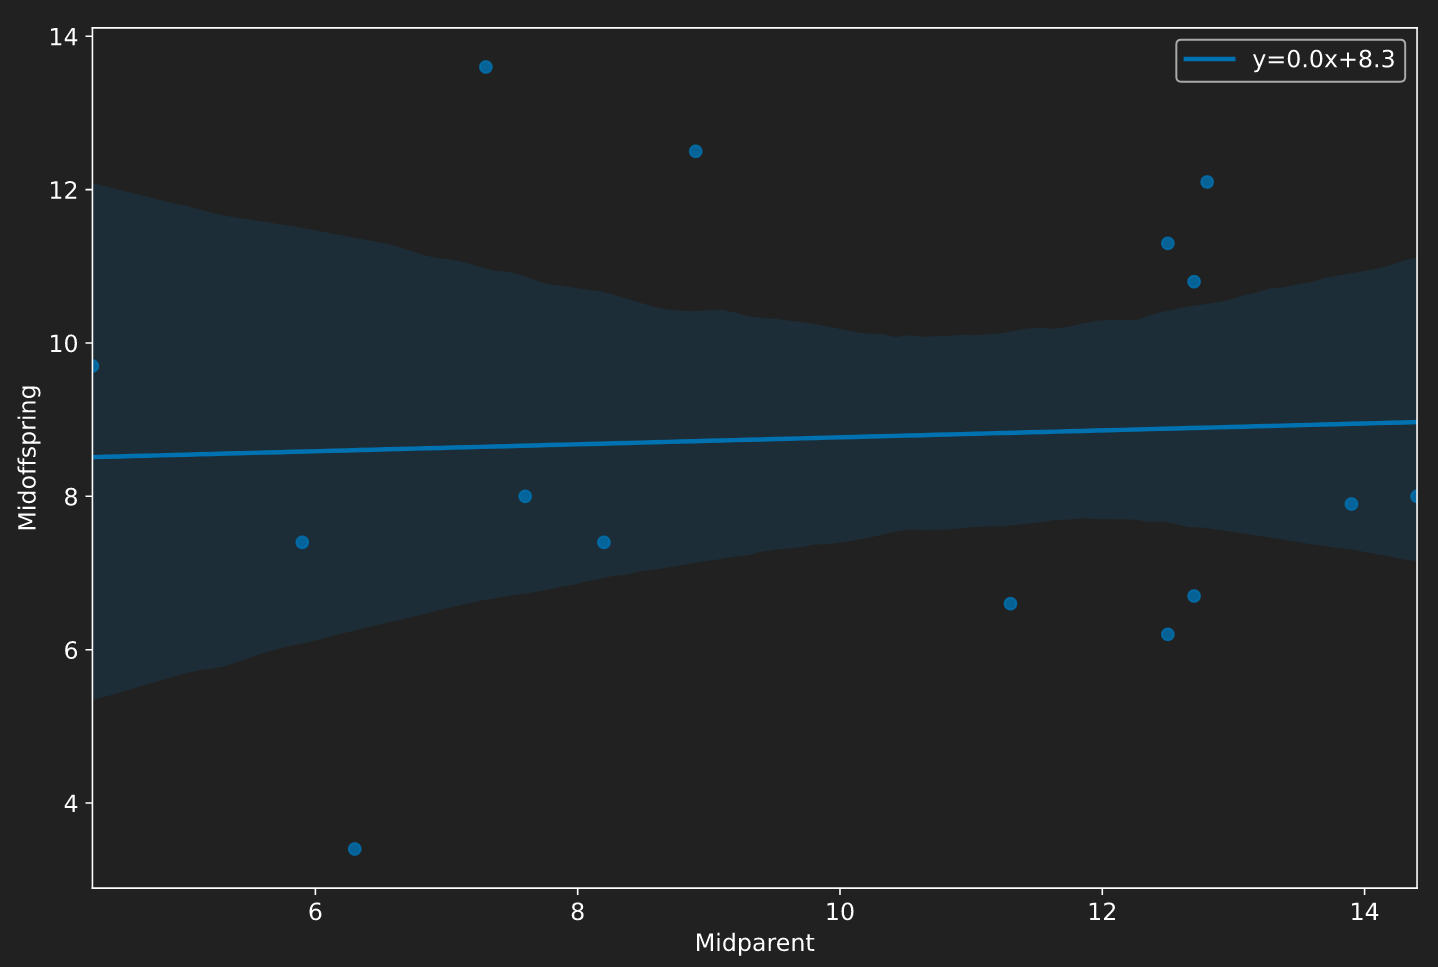
\includegraphics[scale=0.35]{images/heritability.png}
\end{center}
    {\color{G-Moon}\item If she selectively breeds her dogs, will the next generation run substantially faster than the dogs she has now?}
        \begin{itemize}
            \item No, very low heritability, nearly 0. (y=0.0x+8.3)
        \end{itemize}
    {\color{G-Moon}\item What else would you suggest the breeder try if she wants to win more races?}
        \begin{itemize}
            \item Continue to track the midoffspring and midparent speeds, selectively breeding those who tend have a higher heritability ratio in regards to speed
            \item Such a low slope could indicate low heritability of speed, so might be more useful to pursue environmental factors.
        \end{itemize}
\end{enumerate}



%\endgroup
%%%%%%%%%%%%%%%%%%%%%%%%%%%%% Week 5%%%%%%%%%%%%%%%%%%%%%%%%%%%%%





%%%%%%%%%%%%%%%%%%%%%%%%%%%%% Chapter 4 %%%%%%%%%%%%%%%%%%%%%%%%%%%%%
%\begingroup
\clearpage
\section*{Week 4}\phantomsection
\addcontentsline{toc}{section}{\textbf{Week 4}}
\fancyhead[R]{\hyperlink{home}{Week 4}}

\fancyhead[L]{\hyperlink{home}{Molecular Clock}}
\subsection{Molecular Clock}
\begin{align*}
    \textbf{CHEETA EXAMPLE:}\\
    \text{{\color{p-Lush}Divergence: 5.2\%} per 1mya, {\color{g-Fresh} Diversity for this locus: 0.182\%} per [x=time]}\\
    \frac{{\color{g-Fresh}0.182}}{x} = \frac{{\color{p-Lush}5.2\%}}{\num{1e6}}\\
    \num{1.82e5}= 5.2x\\
    x = \frac{\num{1.82e5}}{5.2} = \SI{35000}{yrs}\\ 
    \text{{\color{p-Lush}Divergence: 6.5\%} per 1mya, {\color{g-Fresh}Diversity for this locus: 0.182\%} per [x=time]}\\
    \frac{{\color{g-Fresh}0.182}}{x} = \frac{{\color{p-Lush}6.5\%}}{\num{1e6}}\\
    \num{1.82e5}= 6.5x\\
    x = \frac{\num{1.82e5}}{6.5} = \SI{28000}{yrs}\\ 
    \textbf{DOGS EXAMPLE:}\\
    \text{{\color{p-Lush}Divergence: 7.5\%} per 1mya, {\color{g-Fresh}Diversity for this locus: 1\%} per [x=time]}\\
    {\color{G-Moon}\text{Note: 0.075, and 0.01 converted to \%}}\\
    \frac{{\color{g-Fresh}1}}{x} = \frac{{\color{p-Lush}7.5\%}}{\num{1e6}}\\
    \num{1e6}= 7.5x\\
    x = \frac{\num{1e6}}{7.5} = \SI{133333}{yrs}\\
\end{align*}

\newpage
\fancyhead[L]{\hyperlink{home}{Zika Evolution}}
\subsection{Zika Evolution}
{\color{darklc} Metsky HC et al. 2017. Zika virus evolution and spread in the Americas. Nature 546: 411-415. $\mapsto$}
\subsubsection{Background}
\begin{itemize}
    {\color{G-Moon}\item What was known about Zika virus evolution before this paper was written?}
        \begin{itemize}
            \item Fewer than 100 ZIKV genomes were previously sequenced directly from clinical samples, providing little information about it's epidemiology and evolution.
            \item The virus had a link to birth defects and other neurological complications.
        \end{itemize}
    {\color{G-Moon}\item What were the goals of the authors of this paper?}
        \begin{itemize}
            \item "to gain a deeper understanding of the viral populations underpinning the ZIKV epidemic by extensive genome sequencing."
            \item Understand how sequences are changing and how selection might be acting on the virus.
            \item Where the virus originated.
        \end{itemize}
\end{itemize}

\subsubsection{Methods}
\begin{itemize}
    {\color{G-Moon}\item What taxa were sampled for this study and where specifically were they from?}
        \begin{itemize}
            \item Samples were collected from United States, Guatemala/ El Salvador, Haiti, Dominican Republic, Honduras, Puerto Rico, Martinique, Jamaica, Brazil, and Columbia.
            \item Puerto Rico, Honduras, Columbia, and the Caribbean (includes USA) were the four well supported clades.
        \end{itemize}
    {\color{G-Moon}\item Why was this sampling strategy important to address their goals?}
        \begin{itemize}
            \item Unbiased metagenomic sequencing of 38 samples proved to have insufficient ZIKV RNA for genome assembly, so PCR amplification (110/229 genomes) and hybrid capture (37/66 genomes) had to be used for enrichment.
            \item They had a short sampling period, so deleterious mutations were hard to catch, as well as other changes. They needed a large and diverse set of samples to establish a molecular clock and a substitution rate.
        \end{itemize}
    {\color{G-Moon}\item How was evidence of selection on the Zika virus genome determined?}
        \begin{itemize}
            \item Total of 110 genomes, plus 64 previous published genomes were used in a reconstrued phylogenetic tree based on a molecular clock. 
            \item Each lineage was then traced back to root and used to estimate the substitution rate, which would provide evidence of selection.
            \item Aimed to compare ratio between synonomys and nonsynonymous mutations.
        \end{itemize}
\end{itemize}
\subsubsection{Results}
\begin{itemize}
    {\color{G-Moon}\item Looking at the results shown in Figure 2, explain how the authors arrived at the conclusion that the Zika virus outbreak originated in Brazil.}
        \begin{itemize}
            \item The Brazil ZIKV genomes appear on all deep branches of the tree, and the most recent common ancestor is the root of the tree.
        \end{itemize}
    {\color{G-Moon}\item When did the authors determine the Zika virus outbreak(s) occurred?}
        \begin{itemize}
            \item Early 2014, 95\% confidence interval from August 2013 to July 2014.
        \end{itemize}
    {\color{G-Moon}\item What was the substitution rate for the Zika virus since the outbreak in the Americas?}
        \begin{itemize}
            \item Within-outbreak substitution rate of \num{1.15e-3},  95\% confidence interval of \num{9.78e-4} to \num{1.33e-3}
            \item A 1.3--5 times higher rate than other flaviviruses.
            \item May be higher than expected as samples did not have time for purifying selection produce an effect.
        \end{itemize}
    {\color{G-Moon}\item Why did the authors search for whether there was an excess of nonsynonymous mutations in the Zika virus envelope glycoprotein (nicknamed E)?}
        \begin{itemize}
            \item "Viral surface glycoproteins are known targets for positive selection; mutations in these proteins can confer adaption to new vectors or aid immune escape."
            \item If there was an increased substitution rate it would indicate for selection.
        \end{itemize}
    {\color{G-Moon}\item Was evidence of selection found anywhere in the Zika virus genome? Explain.}
        \begin{itemize}
            \item Adaptive mutations are more likely to be found at high frequency among the nonsynonymous mutations.
            \item Strong evidence for unrestrained diversifying selection was not found due to similar nonsynonymous substitution rates compared to other coding regions.
            \item So no, no strong evidence for selection was found.
        \end{itemize}
\end{itemize}
%\endgroup
%%%%%%%%%%%%%%%%%%%%%%%%%%%%% Chapter 4 %%%%%%%%%%%%%%%%%%%%%%%%%%%%%


%%%%%%%%%%%%%%%%%%%%%%%%%%%%% Week 3 %%%%%%%%%%%%%%%%%%%%%%%%%%%%%
%\begingroup
\clearpage
\section*{Week 3}\phantomsection
\addcontentsline{toc}{section}{\textbf{Week 3}}
\fancyhead[R]{\hyperlink{home}{Week 3}}

\fancyhead[L]{\hyperlink{home}{\textit{Populus} Stimulations}}
\subsection{\textit{Populus} Stimulations}
\begin{enumerate}
    \subsubsection*{Exercise 1: Stimulating Strong Selection}
    {\color{darklc}\item  Describe how the frequency of the \textit{A} allele changes due to strong selection.}
        \begin{itemize}
            \item The frequency of the \textit{A} allele {\color{pos}increases rapidly} due to strong selection.
        \end{itemize}
    {\color{darklc}\item How many generations passed before the \textit{A} allele was fixed or lost?}
        \begin{itemize}
            \item Roughly {\color{o-Sun}60--70} generations.
        \end{itemize}
    {\color{darklc}\item How many generations passed before the \textit{a} allele was fixed or lost.}
        \begin{itemize}
            \item Roughly {\color{o-Sun}60--70} generations.
        \end{itemize}
    \subsubsection*{Exercise 2: Simulating Modereate Selection}
    {\color{darklc}\item Describe how the frequency of the \textit{A} allele changes due to slightly weaker selection.}
        \begin{itemize}
            \item Moderate sigmodal increases in frequency.
        \end{itemize}
    {\color{darklc}\item How many generations passed before the \textit{A} allele was fixed or lost?}
        \begin{itemize}
            \item Roughly {\color{o-Sun}120--130} generations.
        \end{itemize}
    {\color{darklc}\item How many generations passed before the \textit{a} allele was fixed or lost?}
        \begin{itemize}
            \item Roughly {\color{o-Sun}120--130} generations.
        \end{itemize}
    \subsubsection*{Exercise 3: Simulating Weak Selection}
    {\color{darklc}\item Describe how the frequency of the \textit{A} allele changes due to weak selection.}
        \begin{itemize}
            \item {\color{pos}Slightly increasing} exponential curve. 
        \end{itemize}
    {\color{darklc}\item How many generations passed before the \textit{A} allele was fixed or lost?}
        \begin{itemize}
            \item Was not fixed or lost after 1000 generations.
        \end{itemize}
    {\color{darklc}\item How many generations passed before the \textit{a} allele was fixed or lost?}
        \begin{itemize}
            \item Same, neither allele was not fixed or lost.
        \end{itemize}
    {\color{darklc}\item If a generation was equal to 10 years, how many years would it take for the frequency of the \textit{A} allele to double in frequency (from 10\% to 20\%)}
        \begin{itemize}
            \item About 550 generations, so approximately {\color{o-Sun}5,500} years.
        \end{itemize}
\end{enumerate}
%\endgroup
%%%%%%%%%%%%%%%%%%%%%%%%%%%%% Week 3 %%%%%%%%%%%%%%%%%%%%%%%%%%%%%

%%%%%%%%%%%%%%%%%%%%%%%%%%%%% Week 2 %%%%%%%%%%%%%%%%%%%%%%%%%%%%%
%\begingroup
\clearpage
\section*{Week 2}\phantomsection
\addcontentsline{toc}{section}{\textbf{Week 2}}
\fancyhead[R]{\hyperlink{home}{Week 2}}
\fancyhead[L]{\hyperlink{home}{Dog Domesticaion}}
\subsection{Dog Domestication}
\begin{itemize}
    \item Background and Goals
        \begin{itemize}
            {\color{darklc} \item What hypotheses about dog domestication are examined in this paper?}
                \begin{itemize}
                    \item The origin of domestic dogs was the main focus; genetic data suggests East Asia, but other data suggests Europe and Siberia. 
                \end{itemize}
            {\color{darklc} \item  What predictions do these hypotheses make? What would the expected phylogenetic trees look like under each of these hypotheses (i.e. what are the expected topologies)?}
                \begin{itemize}
                    \item The most recent common ancestor would indicate origin and genetic data would help confirm time frame.
                \end{itemize}
        \end{itemize}
    \item Methods
        \begin{itemize}
            {\color{darklc} \item  What taxa were sampled for this study?} 
                \begin{itemize}
                    \item Hypothesis was tested using DNA extracted to trace mitochondrial genomes from 18 prehistoric canids and 20 modern wolves from Eurasian and American origin. 
                \end{itemize}
            {\color{darklc} \item  What gene sequences were used for this study?}
                \begin{itemize}
                    \item Wolves, dogs, including divergent breeds, recently published chinese indigenous dogs, and coyotes. (148 mitochondrial genomes)
                \end{itemize}
            {\color{darklc} \item  What phylogenetic methods were used to reconstruct the phylogenetic tree in Figure 1?}
                \begin{itemize}
                    \item Maximum likelyhood, coalescence, and Bayesian.
                \end{itemize}
        \end{itemize}
    \item Results and Discussion
        \begin{itemize}
            {\color{darklc} \item In Figure 1, which wolf sequence is most closely related to the extant dog clade A, and what geographic region is it from?}
                \begin{itemize}
                    \item Wolves: Switzerland 2 14,500.
                    \item Dogs: Argentina, USA (8,500, 1,000) 
                \end{itemize}
            {\color{darklc} \item In Figure 1, which clade of modern dog sequences has the oldest origin? Approximately how old is this clade?}
                \begin{itemize}
                    \item Dog clade A, Russia, 18,000 years ago.
                \end{itemize}
            {\color{darklc} \item Based upon Figure 1, how many times does it appear that modern extant dogs could possibly have been domesticated?}
                \begin{itemize}
                    \item Figure 1 suggests 4, but the the authors state, {\color{G-Moon}"the inferred recent divergence of clade B from wolves now found in Sweden and Ukraine implies that is might represent a mitochondrial genome introgressed from wolves rather than one established by domestication."}
                \end{itemize}
            {\color{darklc} \item What was the topology of the phylogenetic tree that was recovered, and therefore, which hypothesis was supported?}
                \begin{itemize}
                    \item The findings support the conclusion that legacy of dogs derives from wolves of European origin.
                    \item Analysis of coalescence times support divergence time of >15,000 years ago.
                    \item Past mitochondrial and Y chromosome analysis suggestesd non-European, but had less supported data than these findings.
                \end{itemize}
        \end{itemize}
    \item Conclusions
        \begin{itemize}
            {\color{darklc} \item  What are the major conclusions of the paper?}
                \begin{itemize}
                    \item Three of four modern dog clades are more closely related to sequences from ancient European rather than extant wolves with divergence times >15,000 years ago.
                \end{itemize}
            {\color{darklc} \item  Was the taxonomic sampling sufficient to rule out alternative hypotheses? }
                \begin{itemize}
                    \item Ancient panel did not contain specimens from Middle East or China. No, no ancient dog remains older than 13,000 years are known from those regions.
                    \item The mtDNA sequence tree is well supported, but represents a single genetic locus. Independent loci could offer more power to resolve phylogenetic relations.
                \end{itemize}
        \end{itemize}
\end{itemize}

\clearpage
\fancyhead[L]{\hyperlink{home}{Changes in Speech}}
\subsection{How Farming Reshaped Our Smiles and Our Speech}
\begin{itemize}
    \item Gibbons A 2019; doi: 10.1126/science.363.6432.113
\end{itemize}
\begin{enumerate}
    {\color{darklc}\item What is this news article about?}
        \begin{itemize}
            \item How farming may have reshaped our jaws and thus indirectly influencing how we speak.
        \end{itemize}
    {\color{darklc}\item How could diet change the structure of the jaw?}
        \begin{itemize}
            \item Less wear and tear changed how jaws and teeth developped, creating an overbite with the now less worn down teeth.
        \end{itemize}
    {\color{darklc}\item How could jaw structure change speech patterns of humans?}
        \begin{itemize}
            \item Jaw and teeth placement changes how easy it is to make certain sounds, and overbites made "f" and "v" easier to make.
        \end{itemize}
    {\color{darklc}\item Are these changes in jaw structure permanent? Why or why not?}
        \begin{itemize}
            \item Not likely, if you ate diets similar to early humans your teeth would wear down more and impact from wisdom teeth would minimize overbite. Though, there may have been some lasting selection pressure for a natural overbite.
        \end{itemize}
    {\color{darklc}\item Did natural selection shape these changes in jaw structure? Explain.}
        \begin{itemize}
            \item Not likely, mostly likely from behavior change due to mostly diet change.
        \end{itemize}
    {\color{darklc}\item Can natural selection shape speech patterns? Explain.}
        \begin{itemize}
            \item Yes, sexual selection could be a significant. Or if the change in speech pattern could confer a advantage in communication.
        \end{itemize}
    {\color{darklc}\item Can you think of any parallels with other animals where diet influenced feeding structures?}
        \begin{itemize}
            \item Lots of animals, birds (finches!!), dogs, snakes. Huge impact.
        \end{itemize}
\end{enumerate}
%\endgroup
%%%%%%%%%%%%%%%%%%%%%%%%%%%%% Week 2 %%%%%%%%%%%%%%%%%%%%%%%%%%%%%
\end{document}